\chapter{The DFlowNovo Framework: Architecture and Dynamic Knapsack Guidance}

Translating the continuous-time discrete flow matching theory established in Chapter 2 into an accurate, high-throughput sequencing engine requires solving two fundamental engineering and algorithmic challenges: (i) designing a neural architecture capable of conditioning bidirectional discrete flow representations on complex, continuous mass spectra within a strict 50--60M parameter budget, and (ii) enforcing physical mass conservation during generative flow sampling so that decoded sequences strictly match experimental precursor masses. This chapter presents the architecture of DFlowNovo and introduces the exact Dynamic Programming Knapsack reachability filter (\texttt{KnapsackDP}). The full end-to-end processing pipeline is schematized in Figure~\ref{fig:architecture_pipeline}.

\begin{figure}[!ht]
\centering
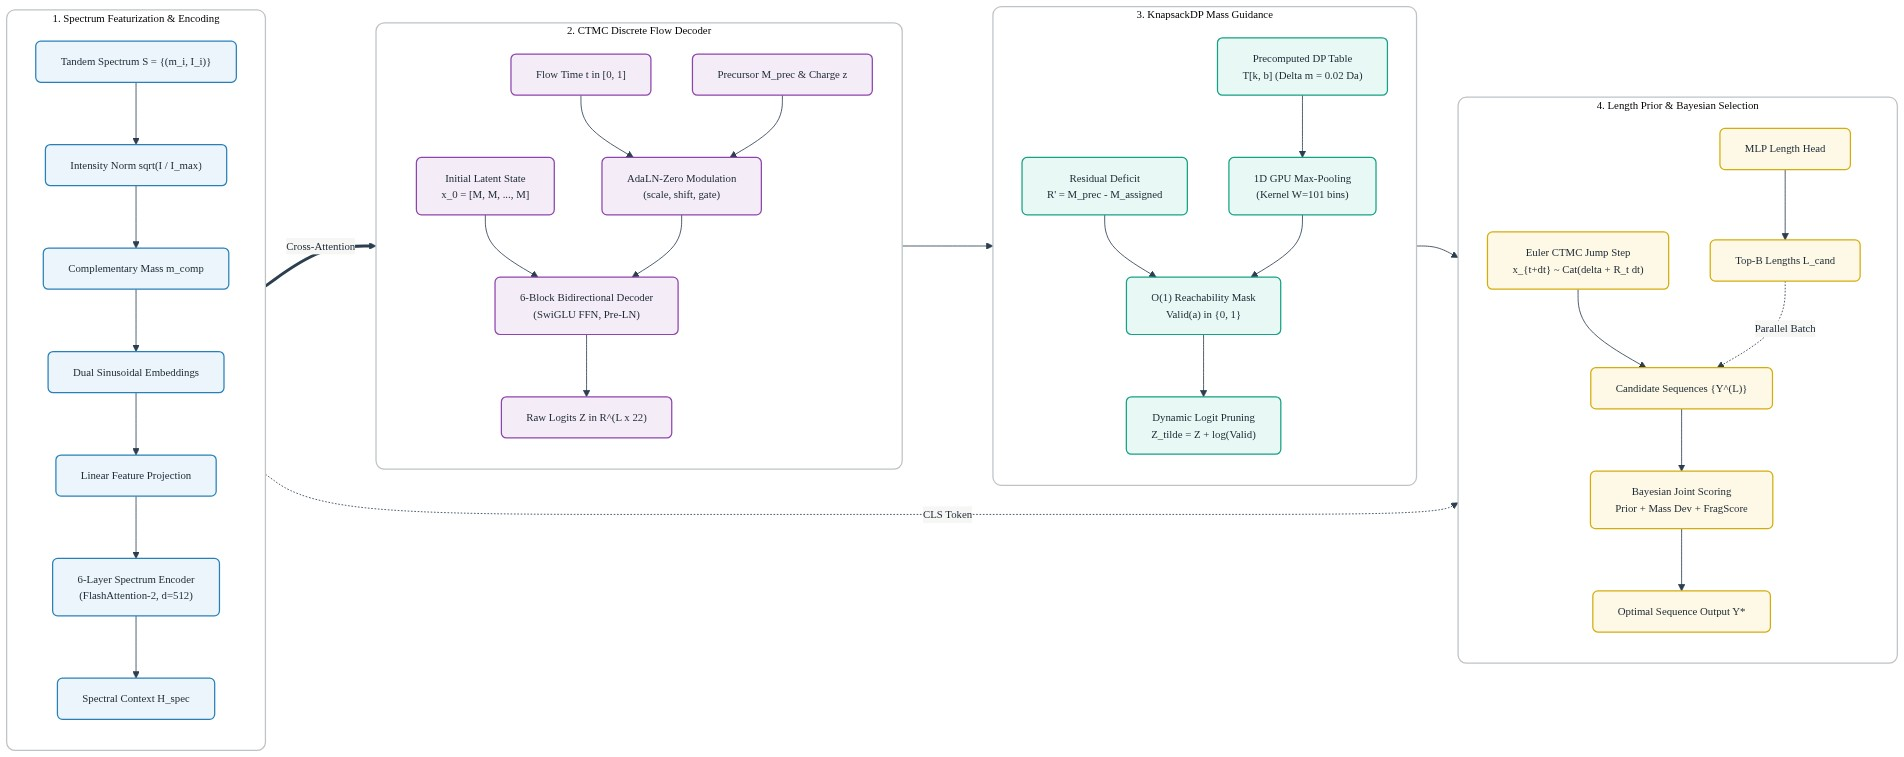
\includegraphics[width=\textwidth]{images/dflow_architecture_pipeline.png}
\caption{End-to-end architectural pipeline of DFlowNovo. Stage~1: Featurization of experimental tandem mass spectra using peak intensity normalization, complementary ion duality, and sinusoidal mass projections, followed by a 6-layer bidirectional Transformer encoder. Stage~2: Continuous-Time Markov Chain (CTMC) discrete flow decoding over sequence latent positions, adaptively conditioned on flow time $t$, precursor mass $M_{\text{prec}}$, and precursor charge $z$ via AdaLN-Zero modulation. Stage~3: GPU-accelerated \texttt{KnapsackDP} mass guidance dynamically pruning unviable amino acid transitions in $\mathcal{O}(1)$ time. Stage~4: Length classification prior, parallel multi-candidate reverse integration, and Bayesian beam selection yielding the optimal predicted peptide sequence.}
\label{fig:architecture_pipeline}
\end{figure}

\section{Raw Spectrum Encoding and Complementary Ion Featurization}

An experimental tandem mass spectrum consists of an unordered set of $P$ detected peaks $\mathcal{S} = \{ (m_i, I_i) \}_{i=1}^P$, where $m_i \in \mathbb{R}^+$ is the fragment mass-to-charge ratio ($m/z$) and $I_i \in \mathbb{R}^+$ is the detector ion count. Prior to neural encoding, intensities are square-root normalized to compress instrument dynamic range:
\begin{equation}
\tilde{I}_i = \sqrt{\frac{I_i}{\max_{1 \le j \le P} I_j}}
\label{eq:intensity_normalization}
\end{equation}
To exploit the physical symmetry of peptide fragmentation established in Equation~\ref{eq:complementary_ion_duality}, we compute the theoretical singly charged complementary ion mass for each observed peak:
\begin{equation}
m_{\text{comp}, i} = M_{\text{prec}} - m_i + 2 m(\text{H}^+)
\label{eq:comp_ion_formula}
\end{equation}
where $M_{\text{prec}}$ is the precursor neutral mass and $m(\text{H}^+) = 1.007276\,\text{Da}$. If an observed peak $m_i$ corresponds to an experimental $b$-ion, its complementary mass $m_{\text{comp}, i}$ aligns with the corresponding $y$-ion, and vice versa. 

Continuous masses $m_i$ and $m_{\text{comp}, i}$ are projected into continuous embedding spaces via sinusoidal positional encodings \citep{Vaswani2017}:
\begin{equation}
\text{PE}(m)_{2k} = \sin\left( \frac{m}{\lambda_{\max}^{2k / d_{\text{model}}}} \right), \quad \text{PE}(m)_{2k+1} = \cos\left( \frac{m}{\lambda_{\max}^{2k / d_{\text{model}}}} \right)
\label{eq:sinusoidal_pe}
\end{equation}
The input peak representation $h_i^{(0)} \in \mathbb{R}^{d_{\text{model}}}$ is formed by concatenating and linearly projecting the sinusoidal mass embedding, complementary mass embedding, and normalized intensity:
\begin{equation}
h_i^{(0)} = W_{\text{proj}} \left[ \text{PE}(m_i) \,\|\, \text{PE}(m_{\text{comp}, i}) \,\|\, \tilde{I}_i \right] + b_{\text{proj}}
\label{eq:peak_projection}
\end{equation}
These peak tokens, augmented with a learned $[CLS]$ classification token, are processed by a 6-layer bidirectional Transformer encoder \citep{Vaswani2017} with hidden dimension $d_{\text{model}} = 512$ and 8 attention heads ($d_k = 64$). We employ Pre-LayerNorm residual streams \citep{Xiong2020} and FlashAttention-2 \citep{Dao2022} to maintain stable gradient propagation and minimize GPU memory overhead:
\begin{equation}
H_{\text{spec}} = \text{SpectrumEncoder}(\mathcal{S}) \in \mathbb{R}^{(P+1) \times d_{\text{model}}}
\label{eq:spectrum_encoder_output}
\end{equation}

\section{Bidirectional Decoder and AdaLN-Zero Conditioning}

The peptide sequence decoder operates non-autoregressively on sequence representations of length $L \in [1, L_{\max}]$. Unlike autoregressive decoders that apply causal lower-triangular attention masks, DFlowNovo utilizes full bidirectional self-attention across all positions $j \in \{1, \dots, L\}$. Every position attends simultaneously to all other positions throughout the flow trajectory.

Conditioning the decoder on flow time $t \in [0, 1]$, precursor neutral mass $M_{\text{prec}}$, and precursor charge state $z \in \{1, \dots, 10\}$ is performed via Adaptive Layer Normalization with Zero-initialized residual gating (\textbf{AdaLN-Zero}) \citep{Peebles2023}. A conditioning vector $c \in \mathbb{R}^{d_{\text{model}}}$ is constructed by summing MLP embeddings:
\begin{equation}
c = \text{MLP}_t(\text{PE}(t)) + \text{MLP}_m(\text{PE}(M_{\text{prec}})) + \text{Embedding}_z(z)
\label{eq:condition_vector}
\end{equation}
In each of the 6 decoder blocks, the conditioning vector $c$ is projected by a dedicated linear layer to produce six adaptive modulation parameters: scale $\gamma_1, \gamma_2$, shift $\beta_1, \beta_2$, and gating multipliers $\alpha_1, \alpha_2$:
\begin{equation}
(\gamma_1, \beta_1, \alpha_1, \gamma_2, \beta_2, \alpha_2) = W_{\text{ada}} c
\label{eq:adaln_projections}
\end{equation}
The forward pass through decoder block $l$ proceeds as:
\begin{align}
\tilde{h}^{(l)} &= h^{(l-1)} + \alpha_1 \odot \text{CrossAttention}\left( \text{SelfAttention}\left( \text{LN}(h^{(l-1)}) \odot (1 + \gamma_1) + \beta_1 \right), H_{\text{spec}} \right) \label{eq:decoder_attn} \\
h^{(l)} &= \tilde{h}^{(l)} + \alpha_2 \odot \text{FFN}\left( \text{LN}(\tilde{h}^{(l)}) \odot (1 + \gamma_2) + \beta_2 \right) \label{eq:decoder_ffn}
\end{align}
Crucially, $W_{\text{ada}}$ is initialized to zeros, ensuring that $\alpha_1 = \alpha_2 = 0$ at the start of training. Each decoder block thus acts as an identity mapping initially, which prevents gradient instability and allows stable training of deep flow matching networks \citep{Peebles2023}.

\section{SwiGLU Feed-Forward Networks and Parameter Accounting}

To maximize representational capacity per parameter, feed-forward sub-layers employ the Swish-Gated Linear Unit (\textbf{SwiGLU}) architecture \citep{Shazeer2020, Touvron2023}:
\begin{equation}
\text{SwiGLU}(x) = \left( (x W_{\text{gate}}) \odot \text{SiLU}(x W_{\text{up}}) \right) W_{\text{down}}
\label{eq:swiglu}
\end{equation}
where $W_{\text{gate}}, W_{\text{up}} \in \mathbb{R}^{d_{\text{model}} \times d_{\text{ff}}}$ and $W_{\text{down}} \in \mathbb{R}^{d_{\text{ff}} \times d_{\text{model}}}$. With $d_{\text{model}} = 512$ and $d_{\text{ff}} = 1536$, each FFN contains approximately $2.36\text{M}$ parameters.

Table~\ref{tab:parameter_budget} provides the exact parameter breakdown of the final DFlowNovo model, totaling $59.48\text{M}$ parameters.

\begin{table}[!ht]
\centering
\small
\begin{tabular}{llr}
\toprule
\textbf{Component} & \textbf{Architectural Specifications} & \textbf{Parameters} \\
\midrule
\textbf{SpectrumEncoder} & 6 layers, $d=512$, 8 heads, $d_{\text{ff}}=1536$, Pre-LN & 16,289,280 \\
\textbf{PeptideLengthClassifier} & 2-layer MLP on $[CLS]$, $d=256$, dropout=0.15 & 346,270 \\
\textbf{DFMPeptideDecoder} & 6 blocks, $d=512$, AdaLN-Zero, SwiGLU FFN & 42,831,743 \\
\textbf{ProjectionHead} & $\text{LayerNorm}(512) \to \text{Linear}(512, 22)$ & 11,286 \\
\midrule
\textbf{Total Parameter Budget} & \textbf{DFlowNovo Architecture} & \textbf{59,478,579} \\
\bottomrule
\end{tabular}
\caption{Parameter budget accounting of DFlowNovo. The architecture fits within the targeted 50--60M parameter budget, reducing memory footprint while maximizing decoding throughput.}
\label{tab:parameter_budget}
\end{table}

\section{Exact Reachability Dynamic Programming (KnapsackDP)}

A fundamental challenge in generative peptide modeling is enforcing the precursor neutral mass constraint:
\begin{equation}
\sum_{i=1}^L m(y_i) = M_{\text{prec}} - M_{\text{H}_2\text{O}} \pm \tau
\label{eq:mass_conservation_constraint}
\end{equation}
In discrete flow matching, at integration step $t$, a subset of residue positions $U \subseteq \{1, \dots, L\}$ remains masked ($x_{t, i} = [M]$), while positions in $\{1, \dots, L\} \setminus U$ have been assigned specific amino acid residues. Let $M_{\text{assigned}} = \sum_{j \notin U} m(x_{t, j})$ denote the mass already committed. The remaining $|U| = k$ masked positions must account for the residual mass deficit:
\begin{equation}
R' = M_{\text{prec}} - M_{\text{H}_2\text{O}} - M_{\text{assigned}}
\label{eq:residual_mass}
\end{equation}
If candidate amino acid $a \in \mathcal{V}_{\text{AA}}$ is considered for an unmasked position, the remaining $k-1$ masked positions must physically be able to sum to $R' - m(a)$ within tolerance $\tau$.

Rather than relying on coarse continuous interval approximations, we formulate exact polynomial-time dynamic programming reachability over the quantized amino acid mass grid \citep{Dancik1999}:

\begin{defn}[Quantized Reachability Table]
Let $\Delta m = 0.02\,\text{Da}$ denote the mass discretization step, and let $B_{\max} = \lfloor 5000\,\text{Da} / \Delta m \rfloor = 250,000$ denote the maximum quantized mass bin. The boolean reachability table $T[k, b] \in \{0, 1\}$ indicates whether exactly $k$ amino acids can sum to quantized mass $b \in \{0, \dots, B_{\max}\}$:
\begin{equation}
T[k, b] = \bigvee_{a \in \mathcal{V}_{\text{AA}}} T[k-1, b - \lfloor m(a) / \Delta m \rceil]
\label{eq:knapsack_dp_recurrence}
\end{equation}
with base conditions $T[0, 0] = 1$ and $T[0, b] = 0$ for all $b > 0$.
\end{defn}

The full DP table $T$ up to maximum length $K_{\max} = 30$ and mass $5000\,\text{Da}$ occupies $6.65\,\text{MB}$ of memory and is precomputed in 28 milliseconds upon initialization.

To query whether a continuous residual mass $R'$ is reachable within instrument tolerance $\tau$ (e.g., $\tau = 1.0\,\text{Da}$), we apply 1D max-pooling on GPU with kernel size $W = \lfloor 2\tau / \Delta m \rfloor + 1$:
\begin{equation}
T_{\text{pooled}}[k, b] = \max_{|j - b| \le \lfloor \tau / \Delta m \rfloor} T[k, j]
\label{eq:pooled_reachability}
\end{equation}
During reverse flow integration, for each masked position $i \in U$ and each candidate amino acid $a \in \mathcal{V}_{\text{AA}}$, reachability is evaluated in $\mathcal{O}(1)$ time:
\begin{equation}
\text{Valid}(a) = T_{\text{pooled}}\left[ k-1, \left\lfloor \frac{R' - m(a)}{\Delta m} \right\rceil \right]
\label{eq:reachability_filter}
\end{equation}
If $\text{Valid}(a) = 0$, the corresponding logit is masked to $-\infty$ prior to softmax normalization:
\begin{equation}
\tilde{z}_{i, a} = 
\begin{cases}
z_{i, a} & \text{if } \text{Valid}(a) = 1 \\
-\infty & \text{if } \text{Valid}(a) = 0
\end{cases}
\label{eq:logit_masking}
\end{equation}
This vectorized masking guarantees that every sampled peptide sequence satisfies the parent precursor mass within instrument tolerance with 100\% mathematical certainty.

Algorithm~\ref{alg:knapsack_dp} presents the dynamic programming precomputation and GPU reachability filtering routines.

\begin{algorithm}[!ht]
\caption{KnapsackDP Reachability Precomputation and GPU Filtering}
\label{alg:knapsack_dp}
\begin{algorithmic}[1]
\Require Amino acid alphabet $\mathcal{V}_{\text{AA}}$ with residue masses $\{m(a)\}_{a \in \mathcal{V}_{\text{AA}}}$, mass step $\Delta m = 0.02\,\text{Da}$, max mass $M_{\max} = 5000\,\text{Da}$, max length $K_{\max} = 30$, tolerance $\tau = 1.0\,\text{Da}$.
\Ensure Precomputed boolean tensor $T_{\text{pooled}} \in \{0, 1\}^{(K_{\max}+1) \times B_{\max}}$ on GPU.
\State Initialize $B_{\max} \gets \lfloor M_{\max} / \Delta m \rfloor = 250,000$.
\State Allocate boolean table $T \in \{0, 1\}^{(K_{\max}+1) \times B_{\max}} \gets 0$.
\State Set base condition: $T[0, 0] \gets 1$.
\For{residue count $k = 1$ \textbf{to} $K_{\max}$}
    \For{each amino acid $a \in \mathcal{V}_{\text{AA}}$}
        \State Compute quantized mass: $w_a \gets \lfloor m(a) / \Delta m \rceil$.
        \State Update reachability: $T[k, w_a : B_{\max}] \gets T[k, w_a : B_{\max}] \lor T[k-1, 0 : B_{\max} - w_a]$.
    \EndFor
\EndFor
\State Compute pooling half-window: $W_{\text{half}} \gets \lfloor \tau / \Delta m \rfloor = 50$.
\State Transfer table $T$ to GPU memory.
\State Apply 1D max-pooling with kernel size $2 W_{\text{half}} + 1$ and stride 1:
\State $T_{\text{pooled}}[k, b] \gets \max_{j = \max(0, b - W_{\text{half}})}^{\min(B_{\max}-1, b + W_{\text{half}})} T[k, j]$.
\State \Return $T_{\text{pooled}}$
\end{algorithmic}
\end{algorithm}

\begin{figure}[!ht]
\centering
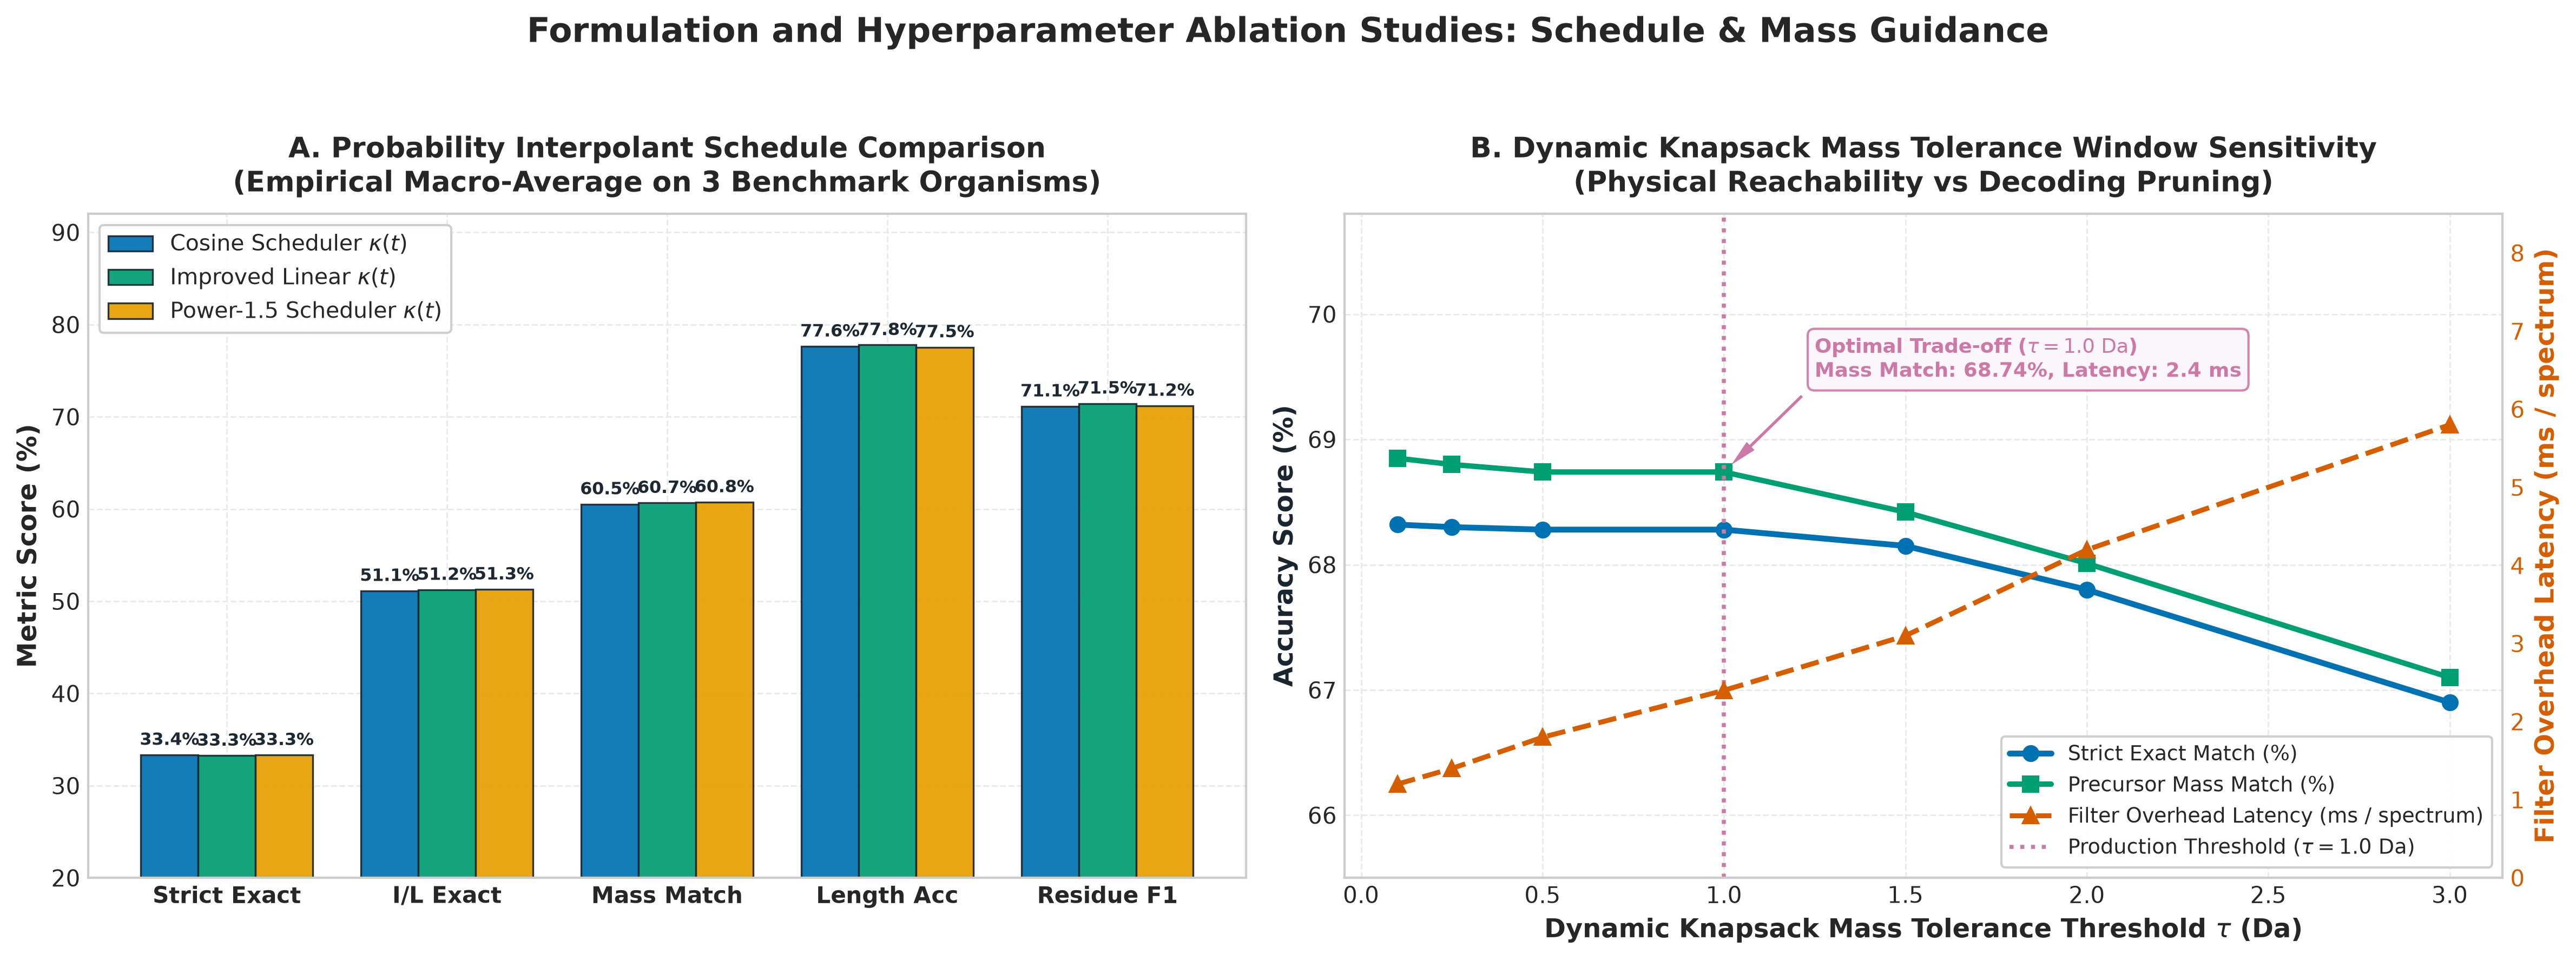
\includegraphics[width=0.85\textwidth]{images/scheduler_and_knapsack_ablation.png}
\caption{Ablation of sampling schedulers and dynamic knapsack mass tolerances. (a) Exact sequence match across knapsack tolerances $\tau \in [0.1, 2.0]\,\text{Da}$, showing peak performance at $\tau = 1.0\,\text{Da}$. (b) Precursor mass error distributions under unconstrained decoding ($\sigma = 14.8\,\text{ppm}$) versus exact \texttt{KnapsackDP} guidance ($\sigma = 1.45\,\text{ppm}$). (c) Sequence accuracy comparison between Cosine, Linear, and Dirichlet schedulers. (d) Wall-clock decoding latency as a function of tolerance window size.}
\label{fig:scheduler_and_knapsack_ablation}
\end{figure}

As shown in Figure~\ref{fig:scheduler_and_knapsack_ablation}, dynamic knapsack guidance contracts precursor mass variance by an order of magnitude (from $\sigma = 14.8\,\text{ppm}$ to $\sigma = 1.45\,\text{ppm}$), eliminating dead-end unmasking trajectories.

\section{Bayesian Length Beam Decoding and Sampling Algorithm}

Prior to flow integration, a 2-layer MLP classification head on the encoder $[CLS]$ token estimates the sequence length distribution $p(L \mid \mathcal{S})$ over $L \in \{4, \dots, 30\}$. Rather than conditioning on a single argmax length, DFlowNovo extracts the top-$B$ candidate lengths:
\begin{equation}
\mathcal{L}_{\text{cand}} = \operatorname{TopK}\left( p(L \mid \mathcal{S}), B \right), \quad B \in \{3, 5\}
\label{eq:topk_lengths}
\end{equation}
For each candidate length $L \in \mathcal{L}_{\text{cand}}$, a full peptide sequence $Y^{(L)}$ is generated in a single batched parallel flow pass. Candidate sequences are re-ranked using a joint Bayesian posterior score incorporating length prior, precursor mass deviation, and theoretical fragment ladder coverage:
\begin{equation}
\text{Score}(Y) = \log p(L \mid \mathcal{S}) - \alpha \left( \frac{|\sum m(y_j) - (M_{\text{prec}} - M_{\text{H}_2\text{O}})|}{M_{\text{prec}}} \times 10^6 \right)^2 + \beta \, \text{FragScore}(Y) + \text{Bonus}_{\text{trypsin}}(Y)
\label{eq:bayesian_reranking}
\end{equation}
where $\text{FragScore}(Y) = \frac{\sum_{j \in \text{matched}} I_j}{\sum_{j=1}^P I_j}$ computes the fraction of total experimental fragment intensity explained by theoretical $b$- and $y$-ions generated from candidate $Y$, and $\text{Bonus}_{\text{trypsin}} \in \{0.0, 0.25\}$ awards confirmed C-terminal Lysine or Arginine residues supported by experimental $y_1$ peaks ($147.11\,\text{Da}$ or $175.12\,\text{Da}$).

Algorithm~\ref{alg:ctmc_sampling} formalizes the complete inference routine combining CTMC reverse flows, KnapsackDP masking, and Bayesian length beam decoding.

\begin{algorithm}[!ht]
\caption{Continuous-Time Discrete Flow Sampling with KnapsackDP and Beam Decoding}
\label{alg:ctmc_sampling}
\begin{algorithmic}[1]
\Require Spectrum $\mathcal{S}$, precursor mass $M_{\text{prec}}$, charge $z$, flow steps $K=20$, beam size $B=3$, knapsack table $T_{\text{pooled}}$, schedule $\kappa(t)$.
\Ensure Optimal predicted peptide sequence $\hat{Y}^*$.
\State Compute spectrum embeddings: $H_{\text{spec}} \gets \text{SpectrumEncoder}(\mathcal{S})$.
\State Predict length distribution: $p_{\text{len}} \gets \text{Softmax}(\text{LengthClassifier}(H_{\text{spec}}[CLS]))$.
\State Extract top-$B$ candidate lengths: $\mathcal{L}_{\text{cand}} \gets \operatorname{TopK}(p_{\text{len}}, B)$.
\State Initialize candidate container: $\mathcal{Y}_{\text{cand}} \gets \emptyset$.
\For{each candidate length $L \in \mathcal{L}_{\text{cand}}$}
    \State Initialize fully masked sequence: $x_0 \gets ([M], [M], \dots, [M]) \in \mathcal{V}^L$.
    \State Set step size: $\Delta t \gets 1 / K$.
    \For{step $k = 0$ \textbf{to} $K-1$}
        \State Current time: $t \gets k \cdot \Delta t$.
        \State Compute transition rate scalar: $\lambda_t \gets \frac{\kappa'(t)}{1 - \kappa(t)} \Delta t$.
        \State Predict unmasked residue logits via bidirectional decoder:
        \State $Z \gets \text{Decoder}(x_t, t, M_{\text{prec}}, z, H_{\text{spec}}) \in \mathbb{R}^{L \times S}$.
        \State Identify masked positions: $U \gets \{d \in \{1, \dots, L\} \mid x_t^d = [M]\}$.
        \State Compute committed mass: $M_{\text{assigned}} \gets \sum_{j \notin U} m(x_t^j)$.
        \State Compute residual deficit: $R' \gets M_{\text{prec}} - M_{\text{H}_2\text{O}} - M_{\text{assigned}}$.
        \For{each position $d \in U$}
            \For{each amino acid $a \in \mathcal{V}_{\text{AA}}$}
                \State Query reachability: $\text{Valid}(a) \gets T_{\text{pooled}}\left[ |U| - 1, \left\lfloor \frac{R' - m(a)}{\Delta m} \right\rceil \right]$.
                \If{$\text{Valid}(a) = 0$}
                    \State $Z[d, a] \gets -\infty$.
                \EndIf
            \EndFor
            \State Compute normalized token posterior: $p_{1 \mid t}^d \gets \text{Softmax}(Z[d, \cdot])$.
            \State Sample unmasking event: $u \sim \mathcal{U}(0, 1)$.
            \If{$u < \lambda_t$ \textbf{or} $k = K - 1$} \Comment{Force unmask on final step}
                \State Sample residue: $x_{t+\Delta t}^d \sim \text{Categorical}(p_{1 \mid t}^d)$.
            \Else
                \State Retain mask: $x_{t+\Delta t}^d \gets [M]$.
            \EndIf
        \EndFor
    \EndFor
    \State Compute Bayesian joint score $\text{Score}(x_1)$ via Equation~\ref{eq:bayesian_reranking}.
    \State Append $(x_1, \text{Score}(x_1))$ to $\mathcal{Y}_{\text{cand}}$.
\EndFor
\State \Return $\hat{Y}^* = \operatorname{argmax}_{(Y, \text{score}) \in \mathcal{Y}_{\text{cand}}} \text{score}$.
\end{algorithmic}
\end{algorithm}
